\documentclass[11pt]{article}

\usepackage[a4paper,margin=1in]{geometry}
\usepackage[T1]{fontenc}
\usepackage[utf8]{inputenc}
\usepackage{lmodern}
\usepackage{microtype}
\usepackage{amsmath,amssymb,amsthm,mathtools}
\usepackage{booktabs}
\usepackage{graphicx}
\usepackage{float}
\usepackage{placeins}
\usepackage{enumitem}
\usepackage[numbers,sort&compress]{natbib}
\usepackage{xcolor}
\usepackage{xurl}
\usepackage[colorlinks=true,linkcolor=blue!55!black,citecolor=blue!55!black,urlcolor=blue!55!black]{hyperref}
\usepackage[nameinlink,noabbrev]{cleveref}

\setlength{\parindent}{1.4em}
\setlength{\parskip}{0.15em}
\setlist{itemsep=0.25em,topsep=0.35em}
\allowdisplaybreaks

\newtheorem{theorem}{Theorem}[section]
\newtheorem{proposition}[theorem]{Proposition}
\newtheorem{lemma}[theorem]{Lemma}
\newtheorem{corollary}[theorem]{Corollary}
\theoremstyle{definition}
\newtheorem{definition}[theorem]{Definition}
\theoremstyle{remark}
\newtheorem{remark}[theorem]{Remark}

\newcommand{\C}{\mathbb C}
\newcommand{\Id}{\mathrm I}
\newcommand{\fl}{\operatorname{fl}}
\newcommand{\up}{\operatorname{up}}
\newcommand{\down}{\operatorname{down}}
\newcommand{\wind}{\operatorname{wind}}
\newcommand{\smin}{s_{\min}}
\newcommand{\norm}[1]{\left\lVert#1\right\rVert}

\hypersetup{
  pdftitle={Outward-Rounded Primal-Dual Residual Enclosures at a Quadratic Band-Merging Map},
  pdfauthor={Liang Wang},
  pdfsubject={Stored-factor floating-point error graphs and conditional Feshbach budgets},
  pdfkeywords={outward rounding, componentwise enclosure, primal-dual residual, Feshbach map, matrix Rouche theorem, floating-point verification}
}

\title{\textbf{Outward-Rounded Primal--Dual Residual Enclosures}\
\textbf{at a Quadratic Band-Merging Map:}\\[0.35em]
\large Stored-Factor Error Graphs, a Normwise False Failure,\\
and Componentwise Recovery}
\author{Liang Wang\\
\small School of Artificial Intelligence and Automation,\\[-0.2em]
\small Huazhong University of Science and Technology, Wuhan 430074, P.R. China\\
\small \texttt{wangliang.f@gmail.com}}
\date{July 2026}

\begin{document}

\maketitle

\begin{abstract}
Primal--dual residual squaring can make a directional Feshbach error
proportional to the product of two residuals, but the residuals reported in
the preceding calculation were ordinary binary64 values near the floating
recurrence floor.  This paper replaces them by outward-rounded enclosures
for an exact finite model defined by the stored binary64 factors.  If
\(M,R,L,\Lambda,V,W\) denote the stored sparse transfer matrix,
peripheral factors, and packet pair, we define exactly
\[
 U=M-R\Lambda L^*,\qquad Q=\Id-VW,
\]
\[
 B=QU^2Q,\quad C=QU^2V,\quad D=WU^2V,\quad E=WU^2Q.
\]
No computed projector or eigensystem is assumed exact beyond this
stored-factor definition.  For \(A_z=z\Id-B\), a base and deep primal pair
\(X_J,X_K\), and a dual approximation \(Z\), set
\[
 r=C-A_zX_K,\qquad s=E^*-A_z^*Z,
\]
and retain the base-consistency term
\(\delta_J=z\Id-D-EX_J-F_J\).  We prove the exact identity
\[
 F-F_J=\delta_J-E(X_K-X_J)-Z^*r-s^*A_z^{-1}r.
\]

Under the standard round-to-nearest model, with no overflow or harmful
underflow, we propagate two nested enclosure geometries through the complete
sparse/dense computation graph.  A normwise scheme stores one Frobenius
radius, whereas a componentwise scheme stores one complex-disc radius per
entry.  Dot products use conservative
\(\gamma_{4k+8}\) bounds for real matrices acting on complex data and
\(\gamma_{16k+16}\) for fully complex products; every bound operation is
rounded outward.  Small packet inverses are certified by a Neumann defect.
The resulting quantities \(\bar\eta\) and \(\bar c\) satisfy
\[
 \norm{F_J^{-1}(F-F_J)}_2
 \leq \bar\eta+\norm{A_z^{-1}}_2\bar c,
\]
and therefore give a downward-rounded conditional inverse budget
\(M_*^-=(1-\bar\eta)/\bar c\).

The normwise audit covers seven stored matrices with
\(2048\leq n\leq204800\) and 32 nodes per contour.  It succeeds at the
first six scales, but gives a transparent false failure at
\(\sigma=10^{-4}\): four nodes have \(\bar\eta\geq1\), with maximum
\(5.66\), although the corresponding floating-centre ratio is only
\(4.97\times10^{-11}\).  Componentwise refinement of the two finest scales
reduces the maximum ratios to \(2.38\times10^{-4}\) and
\(1.32\times10^{-3}\).  At the finest scale it lowers the worst nodal bound
by a factor \(4.29\times10^3\) and restores a minimum conditional budget
\(4.78\times10^{11}\).  A hybrid normwise/componentwise audit has
\(\max\bar\eta=2.33\times10^{-2}\) and
\(\min M_*^-=6.30\times10^8\) across all seven scales.  An independent
63-bit-significand reevaluation consumes at most \(9.30\times10^{-5}\) of
the corresponding componentwise radius.

These results certify outward residual and small-matrix budget calculations
for the stored finite factors, subject to the stated floating-point model.
They do not supply an upper bound for \(\norm{A_z^{-1}}_2\), validate contour
arcs, enclose construction error from the continuous Gaussian kernel, or
prove a root count for the continuous transfer operator.
\end{abstract}

\noindent\textbf{Keywords:} outward rounding; componentwise error;
primal--dual residual; Feshbach map; matrix Rouch\'e theorem; Arnoldi method;
nonnormal resolvent; quadratic map.

\medskip
\noindent\textbf{MSC 2020:} 37E05; 47A10; 47A55; 47B65; 65F10; 65F15;
65G20; 65P30.

\section{Introduction}
\label{sec:introduction}

Goal-oriented error estimation uses an adjoint residual to estimate a small
quantity of interest without first controlling a full state error
\citep{BeckerRannacher2001,GilesSuli2002}.  This is especially natural for
a Feshbach reduction: the quantity of interest is a packet matrix of rank at
most nine, whereas the complement has up to 204800 coordinates and is
strongly nonnormal.  The preceding primal--dual calculation proved that the
unresolved Feshbach term contains the product of a primal and a dual
residual \citep{WangPrimalDual2026}.  Its smallest reported conditional
inverse budget was \(3.35\times10^{24}\).

That number was intentionally not presented as a certificate.  Both
residuals were evaluated in ordinary binary64 arithmetic, often at
\(10^{-15}\)--\(10^{-13}\) relative scale.  A residual near machine
precision can be numerically informative and still be unsuitable for a
proof.  Matrix construction, sparse products, oblique packet removal,
two-step composition, residual subtraction, and small goal solves all
contribute errors.  Moreover, a single global norm can erase the spatial
structure that makes these errors benign.

The present paper resolves this finite-dimensional arithmetic layer.  Its
main contributions are as follows.

\begin{enumerate}
 \item \textbf{A coherent exact stored-factor model.}  The sparse matrix and
 all low-rank factors are treated as exact binary64 numbers.  The blocks
 \(B,C,D,E\) are defined by their exact algebraic composition.  A base
 consistency defect is retained explicitly, so the argument does not assume
 that a floating projected Feshbach matrix is exactly equal to a separately
 reconstructed ambient formula.
 \item \textbf{An outward floating-point calculus.}  Frobenius balls and
 componentwise complex discs are propagated through the entire factor
 graph using standard \(\gamma_k\) estimates \citep{Higham2002}, with all
 scalar and array bounds rounded toward increasing radius.  The proof is an
 induction over the actual operation graph, not an appeal to an unrecorded
 solver tolerance.
 \item \textbf{A certified small inverse interface.}  The packet matrix
 inverse and all products involving it are bounded by a Neumann defect.
 This turns the residual balls into an explicit upper Rouch\'e contribution
 and a downward conditional inverse budget.
 \item \textbf{A resolved false failure.}  The deliberately coarse normwise
 scheme fails at four nodes of the finest contour.  The componentwise
 scheme, with identical centres and no model or parameter change, reduces
 the worst bound by more than three orders of magnitude and restores a
 positive budget.  Thus enclosure geometry, not the floating centre, is the
 limiting object at that scale.
\end{enumerate}

The hierarchy of claims is central.  Exact algebraic identities and
floating-point enclosure lemmas are theorem-level statements under their
explicit arithmetic assumptions.  The seven-scale numbers are reproducible
finite-matrix calculations.  The sampled winding is a diagnostic only.
There is still no validated upper bound for the complement resolvent, no
arcwise continuation of the nodal bounds, and no passage to a continuous or
zero-noise operator.

\section{Exact stored-factor Feshbach identity}
\label{sec:identity}

\subsection{The finite model}

Fix stored binary64 arrays
\[
 M\in\mathbb R^{n\times n},\quad
 R,L\in\mathbb R^{n\times2},\quad
 \Lambda\in\mathbb R^{2\times2},\quad
 V\in\mathbb R^{n\times m},\quad
 W\in\mathbb R^{m\times n}.
\]
The sparse matrix \(M\) is stored in CSR format and \(\Lambda\) is
diagonal.  Define, in exact arithmetic on these stored numbers,
\begin{equation}
 U=M-R\Lambda L^*,
 \qquad Q=\Id-VW.
 \label{eq:stored-uq}
\end{equation}
The notation \(Q\) is convenient, but no exact idempotence is assumed:
rounding in the construction of \(V,W\) is part of the stored data.  Set
\begin{equation}
 B=QU^2Q,
 \quad C=QU^2V,
 \quad D=WU^2V,
 \quad E=WU^2Q.
 \label{eq:stored-blocks}
\end{equation}
For a spectral parameter \(z\), let
\begin{equation}
 A_z=z\Id-B,
 \qquad
 F(z)=z\Id-D-EA_z^{-1}C,
 \label{eq:exact-feshbach}
\end{equation}
whenever \(A_z\) is invertible.  This model is finite and unambiguous.  It
does not claim that the stored factors are exact eigenvectors, exact packet
duals, or exact quadrature data for an underlying continuum operator.

\subsection{Base consistency and primal--dual correction}

Let \(F_J\in\C^{m\times m}\) be a stored base Feshbach matrix, and let
\(X_J,X_K,Z\in\C^{n\times m}\) be stored base primal, deep primal, and dual
approximations.  Define
\begin{align}
 Y&=X_K-X_J, \\
 r&=C-A_zX_K, \\
 s&=E^*-A_z^*Z, \\
 \delta_J&=z\Id-D-EX_J-F_J.
 \label{eq:all-defects}
\end{align}
The consistency term \(\delta_J\) closes a small but important logical gap.
Even when \(F_J\) and \(X_J\) come from the same Arnoldi construction,
their separately rounded reconstructions need not satisfy
\(F_J=z\Id-D-EX_J\) exactly.

\begin{theorem}[Stored-factor primal--dual identity]
\label{thm:stored-identity}
If \(A_z\) is invertible, then
\begin{equation}
 F(z)-F_J
 =\delta_J-EY-Z^*r-s^*A_z^{-1}r.
 \label{eq:stored-pd-identity}
\end{equation}
\end{theorem}

\begin{proof}
Since \(r=C-A_zX_K\),
\(A_z^{-1}C=X_K+A_z^{-1}r\).  Therefore
\[
 F-F_J
 =z\Id-D-EX_J-F_J-E(X_K-X_J)-EA_z^{-1}r.
\]
The first four terms give \(\delta_J\), and
\(s^*=E-Z^*A_z\) implies
\(EA_z^{-1}r=Z^*r+s^*A_z^{-1}r\).
\end{proof}

Define the computable part
\begin{equation}
 \Delta=\delta_J-EY-Z^*r.
 \label{eq:computed-delta}
\end{equation}
Then all unresolved inverse dependence is confined to the bilinear
remainder \(-s^*A_z^{-1}r\).  The identity is exact for arbitrary stored
approximations; small residuals are not needed for its validity.

\section{Outward enclosure calculus}
\label{sec:enclosures}

\subsection{Arithmetic assumptions}

Let \(u=2^{-53}\) and
\begin{equation}
 \gamma_k=\frac{ku}{1-ku}.
 \label{eq:gamma}
\end{equation}
We assume IEEE-754 binary64 round-to-nearest arithmetic
\citep{IEEE7542019}, no overflow, and no underflow large enough to invalidate
the relative-error model.  Every BLAS or sparse reduction is assumed to be
a sequence of correctly rounded elementary operations with no more than the
operation count reserved below.  Fused multiply-add or a tree reduction
only decreases this conservative count.  Bound arithmetic uses
\texttt{nextafter} toward increasing radius after each scalar or array
operation.

For a real matrix times complex data, a length-\(k\) dot product is assigned
\(4k+8\) real operations.  For a fully complex product it is assigned
\(16k+16\).  The first count covers two real dot products and the Euclidean
recombination; the second covers complex multiplication and accumulation.
Complex addition and scalar multiplication use guards \(\gamma_8\) and
\(\gamma_{16}\), respectively.  These constants are intentionally larger
than implementation-specific sharp bounds.

\subsection{Normwise Frobenius balls}

\begin{definition}
A Frobenius ball \([X]_F=(\widehat X,\rho_X)\) represents every matrix
\(X\) satisfying
\[
 \norm{X-\widehat X}_F\leq\rho_X.
\]
\end{definition}

Suppose \(A\) is an exact stored matrix and
\(\alpha_A\geq\norm{|A|}_2\).  If a matrix product has inner dimension
\(k\), the implemented normwise rule is
\begin{equation}
 \rho_{AX}
 =\up\!\left(
 \alpha_A\rho_X+\gamma_{\kappa(k)}\alpha_A
 \norm{\widehat X}_F
 \right),
 \label{eq:normwise-product}
\end{equation}
centred at \(\fl(A\widehat X)\).  The bound \(\alpha_A\) is the smaller of
an outward Frobenius bound and the outward estimate from
\(\norm{|A|}_1\) and \(\norm{|A|}_\infty\).  Sparse products use the maximum
stored row count in \(\kappa(k)\); adjoint sparse products use the maximum
stored column count.

For two uncertain factors, submultiplicativity gives
\begin{align}
 \rho_{XY}=\up\big(&
 \norm{|\widehat X|}_2\rho_Y
 +\rho_X\norm{\widehat Y}_F
 +\rho_X\rho_Y \\
 &+\gamma_{\kappa(k)}\norm{|\widehat X|}_2
 \norm{\widehat Y}_F\big).
 \label{eq:normwise-uncertain-product}
\end{align}
This global geometry is cheap, but every intermediate error is immediately
allowed to point in the worst possible direction.

\subsection{Componentwise complex discs}

\begin{definition}
A componentwise ball \([X]_c=(\widehat X,P_X)\), with \(P_X\geq0\),
represents every matrix \(X\) satisfying
\[
 |X-\widehat X|\leq P_X
\]
entrywise.
\end{definition}

For exact stored \(A\), the componentwise multiplication rule is
\begin{equation}
 P_{AX}=\up\!\left(
 |A|P_X+\gamma_{\kappa(k)}|A||\widehat X|
 \right),
 \label{eq:component-product}
\end{equation}
centred at the same \(\fl(A\widehat X)\).  Positive products used on the
right-hand side are themselves enlarged by division by
\(1-\gamma_{\kappa(k)}\).  For uncertain factors,
\begin{align}
 P_{XY}=\up\big(&|\widehat X|P_Y+P_X|\widehat Y|+P_XP_Y \\
 &+\gamma_{\kappa(k)}|\widehat X||\widehat Y|\big).
 \label{eq:component-uncertain-product}
\end{align}
Addition, subtraction, conjugation, diagonal scaling, and scalar
multiplication are handled entrywise.  Finally,
\begin{equation}
 [X]_c\subseteq
 [X]_F=\left(\widehat X,\ \up\norm{P_X}_F\right).
 \label{eq:component-to-frobenius}
\end{equation}

\begin{lemma}[Local enclosure]
\label{lem:local-enclosure}
Under the arithmetic assumptions above,
\cref{eq:normwise-product,eq:normwise-uncertain-product} enclose the exact
stored-matrix products in Frobenius norm, and
\cref{eq:component-product,eq:component-uncertain-product} enclose them
entrywise.
\end{lemma}

\begin{proof}
The standard dot-product model gives
\(|\fl(A\widehat X)-A\widehat X|
\leq\gamma_{\kappa(k)}|A||\widehat X|\)
\citep{Higham2002}.  Add \(|A|P_X\) for uncertain input.  For two uncertain
factors, expand
\((\widehat X+\Delta X)(\widehat Y+\Delta Y)\), take entrywise absolute
values, and include the centre-product rounding term.  Taking Frobenius
norms and using submultiplicativity gives the normwise formulas.  Outward
rounding of every nonnegative bound operation preserves the inequalities.
\end{proof}

\begin{theorem}[Stored-factor graph enclosure]
\label{thm:graph-enclosure}
Apply either enclosure calculus to the operation graph
\cref{eq:stored-uq,eq:stored-blocks,eq:all-defects,eq:computed-delta}.
Then the returned balls contain the exact stored-factor values of
\(D,C,E^*,r,s,\delta_J,Y\), and \(\Delta\).
\end{theorem}

\begin{proof}
The source factors are radius-zero balls.  Each graph node is an operation
covered by \cref{lem:local-enclosure}; induction over the directed acyclic
graph proves the claim.  Notice that both occurrences of \(U\), both packet
removals, the construction of \(D,C,E^*\), and all final subtractions are
included.
\end{proof}

This is a standard-model verification in the spirit of floating-point
validation methods \citep{MooreKearfottCloud2009,Rump2010}; it is not a
claim that the hardware centre operations were executed under a global
directed-rounding mode.

\section{Small inverse and conditional Rouch\'e budget}
\label{sec:budget}

The packet matrices have order at most nine, so their inverse action can be
certified separately.  Let \(G\) be a stored approximate inverse of
\(F_J\), and let an outward calculation give
\begin{equation}
 q\geq\norm{\Id-F_JG}_F,
 \qquad q<1.
 \label{eq:neumann-defect}
\end{equation}

\begin{proposition}[Neumann inverse/product certificate]
\label{prop:neumann}
Under \cref{eq:neumann-defect},
\begin{equation}
 \norm{F_J^{-1}}_2
 \leq \frac{\norm{G}_F}{1-q}=:\mathcal I_J.
 \label{eq:inverse-upper}
\end{equation}
For any matrix \(H\),
\begin{equation}
 \norm{F_J^{-1}H}_2
 \leq \norm{GH}_F+\mathcal I_Jq\norm{H}_F.
 \label{eq:inverse-product-upper}
\end{equation}
The same formulas remain valid when every right-hand quantity is replaced
by an outward upper enclosure.
\end{proposition}

\begin{proof}
Writing \(D_J=\Id-F_JG\) gives
\(F_J^{-1}=G+F_J^{-1}D_J\).  Rearranging the norm inequality proves
\cref{eq:inverse-upper}; multiplying the identity by \(H\) proves
\cref{eq:inverse-product-upper}.
\end{proof}

Let the graph calculation and \cref{prop:neumann} provide
\begin{align}
 \bar\eta&\geq\norm{F_J^{-1}\Delta}_2,\\
 \bar r&\geq\norm r_2,\\
 \bar w&\geq\norm{F_J^{-1}s^*}_2,
 \qquad \bar c=\up(\bar w\bar r).
 \label{eq:eta-c}
\end{align}

\begin{theorem}[Outward conditional budget]
\label{thm:outward-budget}
For every \(M\geq\norm{A_z^{-1}}_2\),
\begin{equation}
 \norm{F_J^{-1}(F-F_J)}_2
 \leq\bar\eta+M\bar c.
 \label{eq:outward-rouche}
\end{equation}
If \(\bar\eta<1\), define
\begin{equation}
 M_*^-=\down\!\left(\frac{1-\bar\eta}{\bar c}\right),
 \label{eq:downward-budget}
\end{equation}
with the usual infinite value when \(\bar c=0\).  Then any validated
\(M<M_*^-\) is sufficient for the matrix Rouch\'e inequality at that node.
If \(\bar\eta\geq1\), the returned budget is zero.
\end{theorem}

\begin{proof}
Apply \(F_J^{-1}\) to \cref{eq:stored-pd-identity}, group the first three
terms as \(\Delta\), and use
\[
 \norm{F_J^{-1}s^*A_z^{-1}r}_2
 \leq\norm{F_J^{-1}s^*}_2\norm{A_z^{-1}}_2\norm r_2.
\]
The matrix Rouch\'e conclusion follows from the usual strict norm condition
\citep{GohbergSigal1971}.  Downward rounding makes
\cref{eq:downward-budget} conservative.
\end{proof}

The theorem produces an admissible threshold, not the missing inverse upper
bound.  The inverse-information no-go theorem in the preceding paper shows
that nonzero primal and dual residuals cannot remove this requirement in
general \citep{WangPrimalDual2026}.

\section{Seven-scale protocol}
\label{sec:protocol}

\subsection{Centres and factor graph}

The physical centres are reconstructed from the same stored factors and
shift-invariant Arnoldi families used in the preceding contour calculations
\citep{WangContourFeshbach2026,WangDirectionalRouche2026}.  For each noise
scale:

\begin{enumerate}
 \item build the sparse folded Gaussian midpoint matrix and the two stored
 peripheral mode pairs;
 \item build the packet synthesis/analysis pair \(V,W\), then independently
 reconstruct the exact stored-factor blocks \(D,C,E^*\) through the
 enclosure graph;
 \item construct primal and adjoint Arnoldi families to depth \(J+16\);
 \item at 32 stored contour nodes, reconstruct \(X_J,X_{J+16},Z\), enclose
 \(r,s,\delta_J,Y,\Delta\), certify the small inverse products, and compute
 \(\bar\eta,\bar c,M_*^-\);
 \item record the determinant phase of the corrected centre as a sampled
 diagnostic.
\end{enumerate}

The dimensions span 2048--204800, packet ranks span 4--9, and maximum
primal/dual depths span 52--78.  The largest CSR matrix has
67667810 nonzeros.  Every row has at most 333 stored nonzeros; the maximum
column count grows from 664 to 6642.  Across all scales the smallest nonzero
stored magnitude is about \(7.09\times10^{-17}\), no stored input is
subnormal, and all computed centres and radii remain finite.  These checks
support, but do not replace, the no-harmful-underflow assumption.

\subsection{Two enclosure geometries}

The inexpensive normwise graph is run at all seven scales.  Its purpose is
both practical and diagnostic: it shows where loss of direction becomes
fatal.  The componentwise graph is then run at
\(\sigma=2\times10^{-4}\) and \(10^{-4}\), with the same centres, contour,
depths, and factors.  It carries nonnegative radius arrays through two
additional positive products per sparse action.  No contour or tolerance
is retuned after observing the normwise failure.

An independent cross-check casts the \(\sigma=10^{-2}\), node-zero stored
factors to the platform \texttt{longdouble} type, which has a 63-bit
significand on the test machine.  Sparse products are reevaluated by
explicit CSR row reductions rather than the binary64 SciPy kernel.  This is
a diagnostic of enclosure utilization, not part of the formal binary64
proof.

\section{Results}
\label{sec:results}

\subsection{Normwise closure and its boundary}

\Cref{tab:normwise} reports the maximum outward correction ratio and the
minimum downward budget on each 32-node contour.  Relative residual columns
divide the outward Frobenius bound by the Frobenius norm of the corresponding
stored centre block; they are scale diagnostics rather than interval
quotients.

\begin{table}[H]
\centering
\small
\setlength{\tabcolsep}{4.0pt}
\caption{Seven-scale normwise audit.  A zero budget means that at least one
node has \(\bar\eta\geq1\).}
\label{tab:normwise}
\begin{tabular}{@{}rrrrrrrr@{}}
\toprule
\(\sigma\) & \(n\) & \(m\) & \(J/K\) &
\(\max\bar\eta\) & \(\min M_*^-\) &
\(\max\bar r/\norm C_F\) & \(\max\bar s/\norm{E^*}_F\)\\
\midrule
\(10^{-2}\) & 2048 & 4 & 36/52 & \(2.123\!\times\!10^{-6}\) & \(8.924\!\times\!10^{14}\) & \(5.798\!\times\!10^{-9}\) & \(2.111\!\times\!10^{-9}\)\\
\(4\!\times\!10^{-3}\) & 5120 & 5 & 42/58 & \(3.548\!\times\!10^{-5}\) & \(1.190\!\times\!10^{13}\) & \(4.209\!\times\!10^{-8}\) & \(1.101\!\times\!10^{-8}\)\\
\(2\!\times\!10^{-3}\) & 10240 & 6 & 46/62 & \(7.797\!\times\!10^{-4}\) & \(1.596\!\times\!10^{11}\) & \(3.113\!\times\!10^{-7}\) & \(6.060\!\times\!10^{-8}\)\\
\(10^{-3}\) & 20480 & 7 & 50/66 & \(6.359\!\times\!10^{-3}\) & \(5.888\!\times\!10^{9}\) & \(3.543\!\times\!10^{-6}\) & \(3.874\!\times\!10^{-7}\)\\
\(5\!\times\!10^{-4}\) & 40960 & 7 & 54/70 & \(2.325\!\times\!10^{-2}\) & \(6.301\!\times\!10^{8}\) & \(4.253\!\times\!10^{-6}\) & \(4.544\!\times\!10^{-7}\)\\
\(2\!\times\!10^{-4}\) & 102400 & 8 & 58/74 & \(4.388\!\times\!10^{-1}\) & \(4.294\!\times\!10^{6}\) & \(4.660\!\times\!10^{-5}\) & \(2.928\!\times\!10^{-6}\)\\
\(10^{-4}\) & 204800 & 9 & 62/78 & \(5.658\) & \(0\) & \(4.959\!\times\!10^{-4}\) & \(1.840\!\times\!10^{-5}\)\\
\bottomrule
\end{tabular}
\end{table}

The first six scales satisfy \(\bar\eta<1\) at every sampled node.  At the
finest scale, four nodes fail; node 12 at angle \(3\pi/4\) is worst with
\(\bar\eta=5.6575\).  The floating-centre ratio there is only
\(4.9736\times10^{-11}\).  The discrepancy is not caused by a large
computed correction.  It comes from repeatedly replacing structured error
vectors by one adversarial Frobenius direction.  The maximum normwise
residual inflation over the observed centre norm reaches
\(1.79\times10^9\).

\begin{figure}[H]
\centering
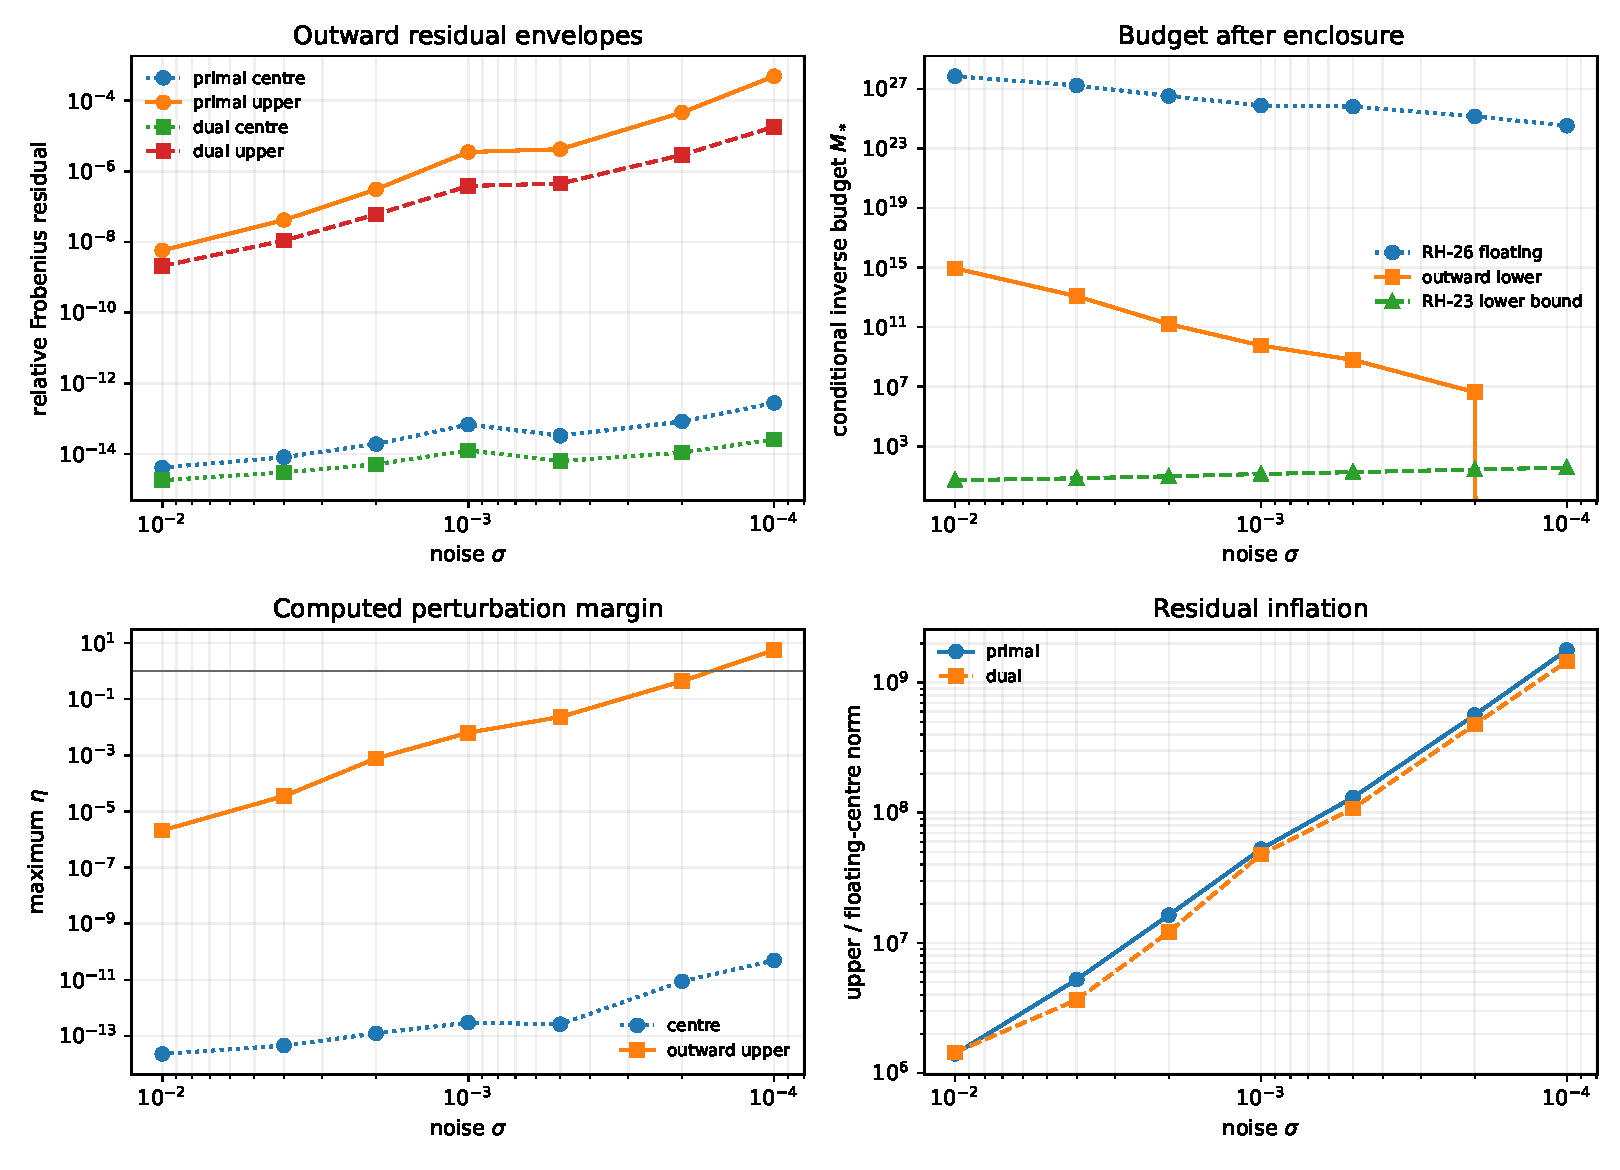
\includegraphics[width=\textwidth]{figures/outward_residual_summary.pdf}
\caption{Normwise seven-scale audit.  Top left: floating-centre residuals
and outward relative bounds.  Top right: RH-26 floating budgets, outward
lower budgets, and the RH-23 one-vector resolvent lower bound shown only as
a scale comparison.  Bottom left: centre and outward correction ratios.
Bottom right: residual inflation caused by the global ball.}
\label{fig:normwise}
\end{figure}

\subsection{Componentwise recovery}

\Cref{tab:componentwise} compares the two geometries at the finest two
scales.  The tightening-factor interval is the minimum and maximum of
\(\bar\eta_{\rm norm}/\bar\eta_{\rm comp}\) over the contour.

\begin{table}[H]
\centering
\small
\setlength{\tabcolsep}{4.0pt}
\caption{Componentwise refinement.  The centres are unchanged.}
\label{tab:componentwise}
\begin{tabular}{@{}rrrrrrr@{}}
\toprule
\(\sigma\) & \(n\) & \(\max\bar\eta_{\rm norm}\) &
\(\max\bar\eta_{\rm comp}\) & tightening & \(\min M_{*,\rm comp}^-\) &
\(\max(\bar r,\bar s)\)\\
\midrule
\(2\!\times\!10^{-4}\) & 102400 & \(4.388\!\times\!10^{-1}\) &
\(2.381\!\times\!10^{-4}\) & \(1.41\!\times\!10^3\)--\(2.46\!\times\!10^3\) &
\(5.379\!\times\!10^{12}\) & \(7.241\!\times\!10^{-8}\)\\
\(10^{-4}\) & 204800 & \(5.658\) &
\(1.317\!\times\!10^{-3}\) & \(2.91\!\times\!10^3\)--\(5.65\!\times\!10^3\) &
\(4.784\!\times\!10^{11}\) & \(3.259\!\times\!10^{-7}\)\\
\bottomrule
\end{tabular}
\end{table}

At the formerly failing node 12, componentwise propagation gives
\[
 \bar r=2.02\times10^{-7},\qquad
 \bar s=3.39\times10^{-8},\qquad
 \norm{\delta_J}_F\leq5.29\times10^{-8},
\]
\[
 \bar\eta=1.3173\times10^{-3},\qquad
 M_*^-=4.7841\times10^{11}.
\]
The nodal ratio is tightened by a factor \(4.29\times10^3\).  The finest
scale is therefore not close to failure once locality is retained.

Using the normwise result for the first five scales and the componentwise
result for the final two gives a seven-scale hybrid audit with
\begin{equation}
 \max_{\sigma,z_j}\bar\eta=2.3254\times10^{-2},
 \qquad
 \min_{\sigma,z_j}M_*^-=6.3013\times10^8.
 \label{eq:hybrid-result}
\end{equation}
The maximum comes from the normwise
\(\sigma=5\times10^{-4}\) layer, not from either componentwise layer.

\begin{figure}[H]
\centering
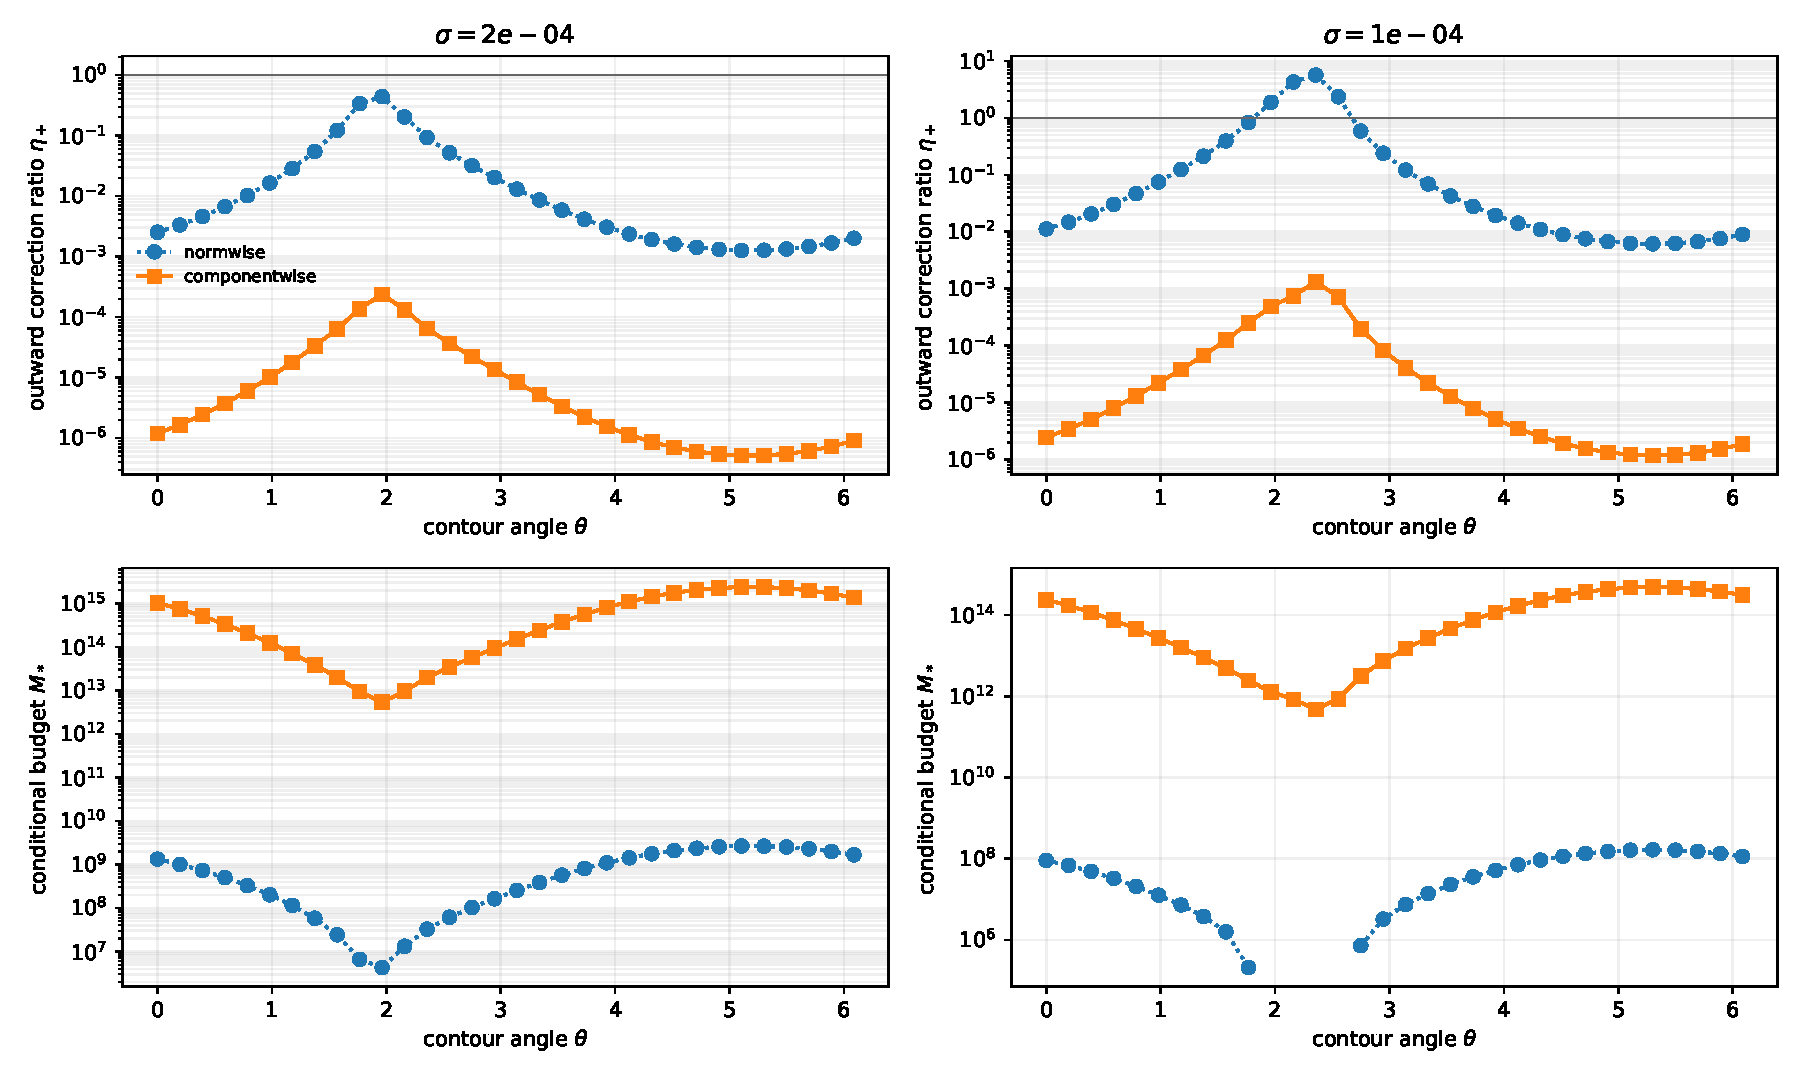
\includegraphics[width=\textwidth]{figures/componentwise_refinement.pdf}
\caption{Normwise and componentwise bounds on the two finest contours.
Top: outward correction ratio; the horizontal line is the Rouch\'e
threshold one.  Bottom: downward conditional inverse budget.  The four
zero-budget normwise nodes at \(\sigma=10^{-4}\) reappear as positive,
large-budget componentwise nodes.}
\label{fig:componentwise}
\end{figure}

\subsection{Cross-checks and sampled centres}

The 63-bit-significand physical reevaluation lies inside every tested
componentwise ball.  Its maximum radius utilization is
\(9.30\times10^{-5}\), attained in the observation-adjoint block; primal,
dual, base-consistency, and total-correction utilizations are all below
\(2.42\times10^{-5}\).  Synthetic unit tests independently cover dense and
sparse multiplication, uncertain products, the full factor graph, the
Neumann inverse certificate, and both ball geometries.

Every corrected centre has sampled winding one on its 32-node contour.  The
largest phase increment in the hybrid audit is \(2.998\), below \(\pi\) but
not accompanied by a validated arc image.  This is reproducible evidence
that the outward corrections do not alter the observed centre winding; it
is not an argument-principle proof.

\section{Evidence hierarchy and limitations}
\label{sec:limitations}

\subsection{What is proved}

The following statements are exact or conditional theorem-level results.

\begin{itemize}
 \item \Cref{thm:stored-identity} is an exact finite-dimensional identity
 for the stored factors, including the base consistency term.
 \item Under the stated standard floating-point model,
 \cref{lem:local-enclosure,thm:graph-enclosure} enclose every listed graph
 output.  Bound arithmetic is outward-rounded.
 \item \Cref{prop:neumann} rigorously reduces the small inverse and inverse
 products to an outward Neumann defect under the same model.
 \item \Cref{thm:outward-budget} is a sufficient nodal matrix-Rouch\'e
 condition for any independently validated complement-inverse upper bound
 below \(M_*^-\).
\end{itemize}

\subsection{What the computations establish}

For the specified stored arrays and software environment, the archived data
show:

\begin{itemize}
 \item six-scale normwise success and a four-node normwise false failure at
 the finest scale;
 \item componentwise recovery at both refined scales, with worst ratio
 \(1.32\times10^{-3}\);
 \item the hybrid bounds in \cref{eq:hybrid-result};
 \item no stored subnormal inputs, finite computed radii, Neumann defects at
 most \(4.60\times10^{-11}\), and a successful independent extended-
 precision diagnostic.
\end{itemize}

\subsection{What remains open}

Five boundaries must not be blurred.

\begin{enumerate}
 \item \textbf{Complement inverse.}  No upper bound for
 \(\norm{A_z^{-1}}_2\) is supplied.  The values \(M_*^-\) are admissible
 thresholds, not estimates of that inverse.  Earlier one-vector resolvent
 lower bounds cannot fill this role.
 \item \textbf{Contour arcs.}  Bounds are evaluated at 32 stored nodes.
 Neither \(\bar\eta\), \(\bar c\), nor the inverse is extended over complete
 arcs.  The sampled winding therefore remains nonrigorous.
 \item \textbf{Matrix construction.}  The binary64 entries of the sparse
 Gaussian matrix and the computed peripheral/packet factors are exact
 inputs to this paper.  Their error relative to exact quadrature,
 eigenspaces, or analytic packet data is not enclosed.
 \item \textbf{Underflow model.}  The stored-data audit rules out subnormal
 inputs and all observed outputs are finite, but a formal hardware-level
 audit of every elementary intermediate is not provided.
 \item \textbf{Operator limits.}  Nothing here proves convergence of the
 finite sections, a small-noise limit, a self-adjoint spectral realization,
 or any statement about zeta zeros.
\end{enumerate}

The extended-precision reevaluation is deliberately not promoted to an
interval proof.  Its role is to detect gross implementation mistakes and
measure conservatism.

\section{Next gate and conclusion}
\label{sec:conclusion}

The arithmetic gate left open by the primal--dual paper has now been crossed
for the stored finite factors.  Ordinary residuals near machine precision
were replaced by outward bounds that include sparse action, low-rank
deflation, oblique packet removal, two-step composition, block
construction, residual subtraction, base consistency, and small inverse
products.  A global Frobenius ball already succeeds through six scales.
Its failure at the seventh is informative rather than terminal: preserving
componentwise locality changes the same node from \(5.66\) to
\(1.32\times10^{-3}\).

The next mathematical gate is now sharply defined.  One needs an arcwise,
validated upper bound for \(\norm{(z\Id-B)^{-1}}_2\), or a direct validated
action bound strong enough to replace it, together with arc extensions of
the small correction quantities.  A uniform bound below
\(6.30\times10^8\) would fit the most conservative hybrid nodal budget, but
this numerical threshold is not itself an existence theorem.  Possible
routes include a validated preconditioned contraction, a block Grushin
inverse, or componentwise interval Krylov actions
\citep{SjoestrandZworski2007,TrefethenEmbree2005,Rump2010}.

The main conceptual result is that certificate geometry is part of the
problem.  A normwise failure can be a proof of excessive information loss,
not evidence against the underlying spectral mechanism.  Here the
componentwise route retains enough structure to keep all seven stored
finite scales open while making the remaining inverse and contour
requirements explicit.

\appendix

\section{Reproducibility and archived artifacts}
\label{app:reproducibility}

The repository directory \citep{WangOutwardCode2026} contains:

\begin{itemize}
 \item \path{src/outward_residuals/enclosures.py}, implementing normwise
 outward balls, Neumann inverse certificates, and downward budgets;
 \item \path{src/outward_residuals/componentwise.py}, implementing
 componentwise complex-disc propagation;
 \item \path{src/outward_residuals/factor_graph.py} and
 \path{componentwise_graph.py}, implementing the complete stored-factor
 primal/dual graph;
 \item \path{experiments/run_outward_residual_audit.py}, the seven-scale
 normwise audit;
 \item \path{experiments/run_componentwise_refinement.py}, the two-scale
 refinement and hybrid summary;
 \item \path{experiments/run_componentwise_longdouble_crosscheck.py}, the
 independent physical extended-precision diagnostic;
 \item seven unit tests, 224 normwise contour rows, 64 componentwise rows,
 scale summaries, source/input hashes, and PDF/PNG figures.
\end{itemize}

From this directory, run
\begin{verbatim}
/root/math/.venv/bin/python -m pytest -q
PYTHONPATH=src /root/math/.venv/bin/python \
  experiments/run_outward_residual_audit.py --reuse
PYTHONPATH=src /root/math/.venv/bin/python \
  experiments/run_componentwise_refinement.py --reuse
\end{verbatim}
The full recomputation is obtained by omitting \texttt{--reuse}; the two
finest scales require the large retained Arnoldi bases.

\section{Operation graph in compact form}
\label{app:graph}

For reference, the primal graph is
\[
 X\mapsto QX\mapsto UQX\mapsto U^2QX\mapsto QU^2QX=BX,
\]
and the adjoint graph reverses these factors.  The static blocks are
\[
 V\mapsto U^2V\mapsto
 \begin{cases}
 WU^2V=D,\\
 QU^2V=C,
 \end{cases}
 \qquad
 W^*\mapsto (U^*)^2W^*\mapsto Q^*(U^*)^2W^*=E^*.
\]
Every arrow is represented by a centre and either a scalar Frobenius radius
or a full componentwise radius array.  The final conversion to
\cref{eq:eta-c} occurs only after \(r,s,\delta_J\), and \(\Delta\) have been
formed.

\bibliographystyle{unsrtnat}
\bibliography{references}

\end{document}
